\documentclass[12pt,]{article}
\usepackage{beamerarticle}
\usepackage[utf8]{inputenc}
\usepackage{hyperref}
\hypersetup{%
  colorlinks=true,% hyperlinks will be coloured
  citecolor={blue!50!black},
  urlcolor={blue!80!black},
  linkcolor=blue,% hyperlink text will be green
  linkbordercolor=blue,% hyperlink border will be red
}

% Math
\usepackage{amssymb,amsmath,amsthm} 
\theoremstyle{plain} % other formats: definition, plain, remark
\newtheorem{proposition}{Proposition}
\newtheorem{define}{Definition}

% Fontfamily
\usepackage{times}%\usepackage{palatino,lmodern, times}

% Page settings
\usepackage[letterpaper, margin=1in]{geometry}
\usepackage{setspace}                           
\onehalfspacing %\doublespacing  % \singlespacing 

% Appendix
\usepackage{appendix}

% Line numbers
%\usepackage{lineno}
%\linenumbers


% Tables
\usepackage{dcolumn}
\usepackage{array,booktabs,longtable,rotating}
\newenvironment{tablenotes}[1][]{
  \begin{minipage}{\textwidth}\emph{Notes:}{\footnotesize #1}
}{\end{minipage}}
\makeatletter
\def\fps@table{htbp}
\makeatother

% Graphics
\usepackage{graphicx,grffile}
\makeatletter
\def\maxwidth{\ifdim\Gin@nat@width>\linewidth\linewidth\else\Gin@nat@width\fi}
\def\maxheight{\ifdim\Gin@nat@height>\textheight\textheight\else\Gin@nat@height\fi}
\makeatother
% Scale images if necessary, so that they will not overflow the page
% margins by default, and it is still possible to overwrite the defaults
% using explicit options in \includegraphics[width, height, ...]{}
\setkeys{Gin}{width=\maxwidth,height=\maxheight,keepaspectratio}
% set default figure placement to htbp
\makeatletter
\def\fps@figure{htbp}
\makeatother

\usepackage{natbib}% plainnat
\bibliographystyle{aer}


\setlength{\emergencystretch}{3em}  % prevent overfull lines
\providecommand{\tightlist}{%
  \setlength{\itemsep}{0pt}\setlength{\parskip}{0pt}}


\usepackage{xcolor}
\usepackage{framed}
\colorlet{shadecolor}{orange!15}
\usepackage{floatrow}
\floatsetup[table]{capposition=top}
\floatsetup[figure]{capposition=top}


% Thresholds, limits, bounds, etc.
\newcommand\deadline{\bar{t}}
\newcommand\target{\underline{y}}

% Competitions
\newcommand\race{\text{race}}
\newcommand\tournament{\text{tour}}

% Cost functions
\newcommand\ctime{c_{t}}
\newcommand\cscore{c_{y}}
\newcommand\cability{c_{a}}
\newcommand\costs{\cability(a_i)\cscore(y_i)\ctime(t_i)}

% Distribution of types
\newcommand\ability{a_i}
\newcommand\marginaltype{\hat{a}}
\newcommand\mtype{\hat{a}}
\newcommand\lotype{\underline{a}}
\newcommand\hitype{\bar{a}}



% Derivatives
\newcommand\dystar{\frac{\partial y^*(x,\target)}{\partial\target}dF_{N:N}(x)}

\title{Races or Tournaments? {[}PRELIMINARY AND INCOMPLETE{]}\thanks{Blasco: Harvard Institute for Quantitative Social Science, Harvard
University, 1737 Cambridge Street, Cambridge, MA 02138 (email:
\href{mailto:ablasco@fas.harvard.edu}{\nolinkurl{ablasco@fas.harvard.edu}}).}}
\author{Andrea Blasco \and Kevin J. Boudreau \and Karim R. Lakhani \and Michael Menietti}
\date{Last updated: 03 May, 2017}

\begin{document}
\maketitle
\begin{abstract}
Contests are often used as incentive schemes to foster innovation. The
typical goal of contest designers is to maximize quality while
minimizing the time it takes to achieve the innovation. This situation
leads to a difficult choice of design made under considerable
uncertainty. In this study, we investigate one key aspect of this
decision that is the way participants compete. Two extreme forms of
competition are considered: the race, where the first to achieve the
innovation wins, and the tournament, where the timing is not important.
We develop a model to characterize under what conditions contest
designers should go for one or the other approach. Then, we report the
results of a field experiment conducted to compare the outcomes of three
alternative competitive situations motivated by theory: the race, the
tournament, and the tournament with a quality requirement. We find that
outcomes in a race are of comparable quality, but are supplied faster.
Based on our model, we also show what would be optimal to do under
several simulated counterfactual situations.

\smallskip\noindent 
JEL Classification: xxx; xxx; xxx.

\smallskip\noindent 
Keywords: xxxx; xxxx xxxx.
\end{abstract}


% Todo notes
%\usepackage[textsize=tiny]{todonotes}
%\newcommand\redmarginpar[1]{\marginpar{\footnotesize{\textcolor{red}{#1}}}}
%\listoftodos[Notes]
\clearpage
\tableofcontents
\setcounter{tocdepth}{2}
\clearpage

\section{Introduction}\label{introduction}

A contest is a competition where participants attempt to win a prize by
investing time and energy in a project. A typical goal for contest
designers is to maximize competitors efforts while minimizing the time
to complete the project. Balancing between these two desirable but often
incompatible goals is often difficult. When contest designers lack full
knowledge of individual costs and skills, design choices are made under
considerable uncertainty. A large economic literature on contest design
offers insights on how to make better resolutions. However, how to
achieve an optimal design is still a largely open question.

We investigate one key aspect of contest design which is the way people
compete. In particular, we contrast two forms of competition with one
another; the ``race,'' where the first to finish an innovation project
wins; and the ``tournament,'' where the best finished project wins.

One is xxx the other is xxxx. To fix ideas about this trade-off, imagine
a government tasked with the design of an innovation contest to progress
on finding a solution to a problem of public health, such as the problem
of antibiotic resistance.\footnote{This example is taken\ldots{}} To
minimize the risks that the threat of xxxx will materialize before a
solution is found, one choice is to design the contest as a tournament
competition with a tight deadline for participants to provide their
solutions. However, if the duration of the competition is too low, a
tournament may give insufficient incentives resulting in inadequate
solutions. Alternatively, the government can set up a race competition
with a prize being awarded to the first competitor who achieves, or goes
beyond, a minimum quality threshold. Here the problem of accelarating
the timing of innovation should not be a big issue but competitors may
work inefficiently, as they have no incentives to exceed the minimum
threshold. Clearly, fixed the prize structure, both approaches have
specific advantages and limitations. However, xxxx.

In the present study, we shed light on the conditions under which
contest designers should choose between a race and a tournament
competition. We proceed in two ways. First, we develop a contest model
that encompasses both the race and the tournament in a single framework.
Exploring the duality of the model, we compare equilibrium behaviors
under both regimes and characterize the optimal choice (i.e., the setup
that maximizes the utility of the contest designer). Then, we design and
execute an experiment to test the implications of the theory in the
field, providing policy recommendations.

Regarding to the modeling, we adapt the contest model introduced by
\citet{moldovanu2001optimal}. Contests have an all-pay structure by
which participants pay an immediate cost for an uncertain future reward.
We generalize by allowing participants to choose the timing and quality
of the innovation at once. This decision is made under the uncertainty
of the costs of the rivals, which are privately observed by the agents.
The contest designer is modeled as an extra agent with preferences for
both time and quality. Following the analysis of the model model, we
show that the optimal design depends on the number of participants and
the concavity of their cost function.

The field experiment was conducted at the end of 2016. The context of
the experiment was an online programming competition. In a programming
competition, participants compete writing source code that solves a
given problem for winning a monetary prize. We worked together with
researchers from the United States National Health Institute (NIH) and
the Scripps Research Institute (SCRIPPS) to select a challenging problem
for the contest. The selected problem was based on an algorithm called
BANNER built by NIH \citep{leaman2008banner} that uses expert labeling
to annotate abstracts from a prominent life sciences and biomedical
search engine, PubMed, so disease characteristics can be more easily
identified. The goal of the programming competition was to improve upon
the current NIH's system by using a combination of expert and non-expert
labeling, as described by \citet{good2014microtask}. The competition was
hosted online on the platform Topcoder.com (about 1M registered users in
2016). Top submissions were awarded monetary prizes ranging between
\$100 to \$5000 for a total prize pool of more than \$40,000.

Our intervention consisted in sorting at random participants into
independent virtual rooms of 10 or 15 people. These virtual rooms were
then randomly assigned to one of three different competitive settings: a
race, a tournament, and a tournament with a reserve score, which is the
lowest acceptable score by the platform for a submission to be awarded a
prize.

We find that xxxxx {[}participation in the tournament is xxx compared to
the race the reserve.{]}

We also find that xxxx {[}submission are quicker in a race, whereas are
equally distributed at the end of the competition in the the tournament
and in the tournament with quality requirement.{]}

Another interesting finding is that xxxxx {[}No evidence trade-off
between a race and a tournament in terms of higher scores vs faster
submissions. We do find that scores are higher in the tournament but we
do not find a strong trade-off in the sense that race had comparable
good quality solutions than the tournament.{]}

\section{Literature}\label{literature}

This paper is related to the contest theory literature
\citet{dixit1987strategic} \citet{baye2003strategic},
\citet{parreiras2010contests}, \citet{moldovanu2001optimal},
\citet{moldovanu2006contest}, \citet{siegel2009all},
\citet{siegel2014contests}. It also relates to the literature on
innovation contests \citet{taylor1995digging}, \citet{che2003optimal}.
And the personnel economics approach to contests \citet{lazear1981rank},
\citet{green1983comparison}, \citet{mary1984economic}.

Empirically, \citet{dechenaux2014survey} provide a comprehensive summary
of the experimental literature on contests and tourments. Large body of
empirical works have focused on sports contests
\citet{szymanski2003economic}. More recently, inside firms (xxx) and
online contest (xxxx).

This paper is also related to the econometrics of auctions
\citet{paarsch1992deciding}, \citet{laffont1995econometrics},
\citet{donald1996identification} and more recently
\citet{athey2011comparing}, \citet{athey2002identification}, and
\citet{athey2007nonparametric}.

An extensive literature has discussed the reasons why contests are
sometimes preferred to other forms of incentives (e.g., individual
contracts). Typically, contests reduce monitoring costs {[}xxx{]},
incentivize production with common risks {[}xxx{]}, and deal with
indivisible rewards {[}xxxx{]}, among others. While there is not much
debate on why contests should be used, the issue of how to effectively
design and deploy a contest still attracts much research.

Several aspects of contest design have been investigated, including the
optimal prize structure {[}XXX, xxxx, xxxx{]}, number of competitors
{[}XXX, XXX{]}, and imposing restrictions to competition such as minimum
effort requirements {[}XXX, XXX{]}. Also, a great deal of theoretical
models of races and tournaments have been developed and applied to a
wide range of economic situations including patent races {[}xxx{]}, arms
races {[}xxx{]}, sports {[}xxx{]}, the mechanism of promotions inside
firms {[}xxxx{]}, sales tournaments {[}xxxx{]}, etc.

\citet{harris1987racing}, \citet{grossman1987dynamic} investigate the
dynamics issues patent races where the interest is how firms compete for
a patent. \citet{bimpikis2014designing} looks at the problem of how to
design an information structure that is optimal when the contest is a
race and innovation is uncertain (encouragement and competition effect).
In the laboratory, \citet{zizzo2002racing} finds poor support to
predictions of dynamic xxxx. In general we do not know much about the
dynamic aspect of contests.

The duality. As pointed out by \citet{baye2003strategic}, many of these
models of tournament and race competitions are specific cases of a more
general ``contest games.'' And sometimes it is possible to design one or
the other in a way to exploit a ``duality.'' In other words, in theory,
a competition can be designed as a tournament to do xxx or as a race to
do xxx. While theoretically very useful, how to exploit this duality in
practice remains largely unknown. Lack of data. As before, xxxx. The
main challenge is self-selection. The answer to this optimal design
question relates to the cost function of agents with respect to ``time''
and to ``effort.'' It is hard to say which solution is better. However,
it is easier to tell whether you should have one prize or multiple
prizes.

\section{The model}\label{the-model}

We now generalize the contest game introduced by
\citet{moldovanu2001optimal} to a situation where players simultaneously
decide \(i)\) the quality and \(ii)\) how fast to produce a given
output. Then we explore the problem of revenue maximization faced by a
contest designer with preferences for both quality and time.

\subsection{Basic setup}\label{basic-setup}

A generalized contest game is an n-player game with asymmetric
information in which each player (\(i=1,..., n\)) competes against the
others to win a prize. Players assign a nonnegative value \(v_k\) to
each prize (\(k=1, ..., q\)) that is decreasing in the prize rank
(\(v_1\geq v_2\geq ...\geq v_q\)). Each player's strategy consists in
choosing an output quality \(y_i\) and a timing \(t_i\) both nonnegative
numbers that determine player \(i\)'s probability \(p_{k}(y_i, t_i)\) of
winning a prize \(k\).

Each player incurs a production cost \(c_i\) that is shaped by a cost
function \(C(\cdot)\) which is increasing in quality and decreasing in
timing. The cost function also depends on an individual ability
parameter \(a_i\) that is private information of each player and that is
drawn at random from a common distribution \(F\) on a finite interval
\([\lotype, \hitype]\) with \(\lotype>0\).\footnote{This assumption
  rules out common parametric distributions like the log-normal and
  forces us to focus the analysis on beta-type distributions. However,
  results do not hinge on this particular assumption.} For simplicity,
we assume the cost function is multiplicative:

\begin{equation}
  C(a_i, y_i, t_i) = c_a(a_i) c_y(y_i) c_t(t_i)
\end{equation}

with \(c_a(\cdot)\) and \(c_t(\cdot)\) being monotonic decreasing
functions (the higher the ability or the time to complete, the lower the
cost) and \(c_{y}(\cdot)\) being a monotonic increasing function (the
higher the quality, the higher the cost). We impose additional
conditions to ensure nonnegative costs \[
    c_{a}(\hitype)>0, c_{t}(\lotype)>0, \text{ and } c_{y}(\lotype)\geq 0.
\]

Player \(i\)'s payoff is then

\begin{equation}
  \label{expected payoff}
  \pi_i = \sum_{k=1}^{q} p_{k}(y_i, t_i) v_k - C(a_i, y_i, t_i). 
\end{equation}

And we can denote a (generalized) contest game \(G\) by

\begin{equation}
G \equiv \left\{
    n, q, \{v_k\}_{k=1}^{q},  F, C, \{p_{k}\}_{k=1}^{q} 
  \right\}.
\end{equation}

When players have to successfully meet a given deadline and/or satisfy a
minimum quality level to be eligible to win a prize, we say that the
contest game \(G\) has a minimum-entry requirement. Let \(\deadline>0\)
be the deadline and \(\target\geq 0\) the required minimum performance.
A game \(G\) has a minimum-entry requirement when, for every prize \(k\)
and player \(i\), the probability \(p_{k}(\cdot, \cdot)=0\) when player
\(i\)'s quality is below a target level \(q_i < \target\) or the timing
to completion is above a given deadline \(t_i>\deadline\). To simplify
exposition, we further use the convention that whenever the deadline is
not met \(t_i> \deadline\) then the output quality is zero \(y_i=0\),
and whenever the required quality is not met \(y_i<\target\) then the
time of completion is above the deadline \(t_i = \infty\). This simply
ensures that when one of the entry-requirements is not met by a player,
the player has a zero probability of winning a prize.

Using the above notation, we define a tournament as a contest game with
the following characteristics.

\begin{definition}[Tournament] \label{tournament}
Let $y_{(1:n-1)}, ..., y_{(n-1:n-1)}$ denote the order statistics of the $y$'s for the $n-1$ opponents of player $i$. A tournament is a contest game $G$ with a minimum-entry requirement $\deadline>0$ where player $i$'s probability of winning a prize is zero when $t_i > \deadline$. Otherwise, when $t_i\leq\deadline$, the probability is 
\begin{equation}
  p_{i, k} =
  \begin{cases}
    \Pr(y_i > y_{n-1:n-1}) & \text{if }k=1\\
    \Pr(y_{n-k+1:n-1} > y_i > y_{n-k:n-1}) & \text{if }k>1.
  \end{cases}
\end{equation}
\end{definition}

In other words, the tournament corresponds to a special case of a
contest game with minimum-entry requirement in which players have a
deadline to meet and the player having achieved the highest output
quality within the deadline gets the first prize, the player having
achieved the second highest output quality gets the second prize, and so
on.

In a similar way, we describe a race as a contest game with the
following characteristics.

\begin{definition}[Race] Let $t_{(1:n-1)}, ..., t_{(n-1:n-1)}$ denote the order statistics of the $t$'s for the $n-1$ opponents of player $i$.  A race is a contest game $G$ with a minimum-entry requirement $\target>0$ where player $i$'s probability of winning a prize is zero if $y_i < \target$. Otherwise, when $y_i\geq \target$, the probability is
\begin{equation}
  p_{i, k} =
  \begin{cases}
    \Pr(t_i < t_{1:n-1}) & \text{if }k=1\\
    \Pr(t_{1-k:n-1} > t_i > t_{k:n-1}) & \text{if }k>1.
  \end{cases}
\end{equation}
\end{definition}

That is, the race corresponds to a special case where the player being
the first to complete a job with a minimum quality gets the first prize,
the player being the second to complete a job with a minimum quality
gets the second prize, and so on.

\subsection{Equilibrium}\label{equilibrium}

In this section, we solve the model for the equilibrium actions of
players. We assume throughout that there are only two prizes of total
value normalized to one, where the fraction \(\alpha\geq 1/2\) goes to
the first placed competitor and \(1-\alpha\) goes to the second placed
competitor. We also let \(F_{r:n}\) and \(f_{r:n}\) be the distribution
and density function of the \(r^{th}\) order statistic (i.e., the
\(r^{th}\) lowest realization) of \(n\) draws from the ability
distribution (i.e., the \(a\)'s).

\subsubsection{Equilibrium in a
tournament}\label{equilibrium-in-a-tournament}

Because the probability of winning a prize in a tournament is not
affected by the completion time (as soon as the deadline is met),
picking a completion time equal to the deadline (\(t_i=\deadline\)) is a
(weakly) dominant strategy for each player. Hence, from the point of
view of the contest designer, imposing a more distant deadline has the
same effect as a reduction in the marginal costs for everyone (i.e.,
proportional to the cost \(\ctime(\deadline)\)). {[}Alternatively, it
can be seen as a reduction in the total value of prizes.{]}

Following \citet{moldovanu2001optimal}, the (unique) symmetric
equilibrium for each player \(i\) is the timing \(t_i^*=\deadline\) and
the output quality \(y_i^*=y^*(a_i)\) with the function

\begin{equation} \label{ystar}
y^*(a_i) = 
    \cscore^{-1}
    \left[\cscore(\target) 
    + \frac{1}{\ctime(\deadline)}
    \left(\alpha \int_{a_i}^{\hitype} A(z) dz
      + (1-\alpha) \int_{a_i}^{\hitype} B(z)  dz
    \right)
    \right]
\end{equation}

where

\begin{equation}
  A(x) = \frac{1}{c_{a}(x)} f_{(n-1:n-1)}(x)
\end{equation}

and

\begin{equation}
  B(x) = \frac{1}{c_{a}(x)} \left\{
      \left[1- F_{(n-1:n-1)}(x)\right]f_{(n-1:n-2)}(x)
      + f_{(n-1:n-1)}(x) F_{(n-1:n-2)}(x)
    \right\}.
\end{equation}

An important property of \eqref{ystar} is that it has its upper bound in
XXXX and lower bound in \(y^*(\lotype) = 0\). Also, equilibrium output
quality is monotonic increasing in the agent's ability
\citep[see][]{moldovanu2001optimal}. Thus, using \(\phi\) to denote the
inverse function, the above equilibrium strategy is obtained by solving
the first-order differential equation:

\begin{align}
    \label{foc0}
0 = & \alpha f_{(1:N-1)}(\phi) \phi^{\prime} 
    + (1-\alpha)\phi^{\prime}\{[1 - F_{(1:N-1)}(\phi)]f_{(1:N-2)}(\phi) + \nonumber\\
    & + f_{(1:N-1)}(\phi) F_{(1:N-2)}(\phi)\} - c_{a}(a) c_{y}(\target) c_{t}^{\prime}(t_i)
\end{align}

with boundary condition \(\phi(0) = \lotype\) (i.e., the lowest-ability
competitor's optimal output quality is zero).

Also, monotonicity of the equilibrium output quality implies that, for
every \(i=1, ..., n\), the equilibrium expected payoff from the contest
\(\pi_i^*\) depends on the rank of the player's ability relative to the
others. That is, the equilibrium payoff is \(\pi_i^*=\pi^*(a_i)\) with

\begin{equation} 
    \pi^*(a_i) = \alpha F_{n:n}(a_i) + (1-\alpha)[1-F_{n:n}(a_i)] F_{n-1:n-1}(a_i)  
    - C(y^*(a_i), \deadline, a_i),
\end{equation}

where \(\pi^*(0) = 0\) and
\(\pi^*(\hitype) = \alpha - C(y^*(\hitype), \deadline, \hitype)>0\).

\subsubsection{Equilibrium in a race}\label{equilibrium-in-a-race}

In a similar way, one can derive the equilibrium strategy in a race.
Because any quality that is below the minimum-entry requirement
\(\target\) will give a zero probability of winning and any quality that
is above \(\target\) is costly but gives a constant probability of
winning, player \(i\)'s choice of optimal quality \(y^*\) is either zero
(with \(t_i=\deadline\) by convention) or \(y^*=\target\).

The (unique) symmetric equilibrium for player \(i\) is the xxxxx when
\(xxxx\) and xxxx.

\begin{equation}
t^* = 
    XXXX
\end{equation}

where

\begin{equation}
  A(x) = XXXX
\end{equation}

and

\begin{equation}
  B(x) = XXXX.
\end{equation}

An important property of XX is that \(y^*(a_i)\) has its upper bound in
XX and lower bound in XX. Also, equilibrium output quality is monotonic
increasing in the agent's ability \citep[see][]{moldovanu2001optimal}.
Thus, for every \(i=1, ..., n+1\), the equilibrium expected reward
depends only on the rank of his ability relative to the others. Using
\({F_{A_{r:n}}}\) to denote the distribution of the \(r\)'th order
statistic of abilities gives

Hence, by setting to zero and solving for the ability, gives the
marginal ability \({\underline a}\) as

\begin{equation}
  {\underline a}= h(n, V, F_A, C, d).
\end{equation}

\subsubsection{Tournament vs races}\label{tournament-vs-races}

By comparing equilibrium xxx and xxx, we find that the race and the
tournament do not (ex-post) dominate one another with respect to output
quality. Whereas the race always dominates the tournament with respect
to completion time. {[}This is only when the deadline is the same.
Otherwise, there's always xxxx.{]} This result is stated below.

\begin{proposition}
There always exist an interval of abilities where the output quality is higher in the race than in the tournament. By contrast, every player takes less completion time in the race than in the tournament.
\end{proposition}

\begin{proof}
Marginal type has utility zero in a race but the same type has a strictly positive utility in the tournament. Since probability of winning is not different in the race or the tournament (the bid is a monotonic transformation of the individual ability or, in other words, rankings are virtually the same), expected payoffs in equilibrium differ only in the cost functions. Hence, to be an equilibrium, the player in the tournament should bid less than the player in the race to earn a strictly positive expected payoff. 
\end{proof}

Let's make an example.

\begin{verbatim}
p <- plnorm   # pdf individual abilities 
r <- rlnorm   # Simulate individual abilities
cy <- function(x) x^2 # Cost function performance
ct <- function(x) 2*exp(1-x)  # Cost function timing 
\end{verbatim}

FIGURE 1. Equilibrium bids in a race and a tournament.

Implications. The above proposition applies only if the target is higher
in a race than in a tournament. But what if the two competitions had the
same target ? In that case, tournaments and races have the same marginal
type. Therefore, the performance of players in the tournament with
reserve are always non-lower than those in the race. This does not imply
that it is optimal to set the target. On the contrary, we will show that
it is optimal to set an optimal target in a tournament that is below the
optimal target in a race. Next section.

\subsection{The contest designer's
problem}\label{the-contest-designers-problem}

Let us now focus on the contest designer's problem. Imagine the contest
designer can choose the competition format to be either the race or the
tournament. Imagine all other aspects of design are given. The prize
structure \(\alpha\) has been already chosen. There is a deadline
\(\deadline\), which is the same in both competition formats. {[}The
quality requirement \(\target_c\) in the tournament is smalle than that
in the race \(\target_\race > \target_\tournament\)){]} We will relax
this assumption later to consider a more general setting where these
variables are also part of the contest designer's problem.

The contest designer has an objective function that is increasing in the
expected quality of the winning solution and decreasing in the
corresponding time to completion. Here, to do not complicate exposition,
we assume that the contest designer cares about the winning submission
only: second placed efforts are not considered. {[}If the principal
values the diversity of the solutions \ldots{} but we assume it does
not.{]}

XXX EQUATION XXXX

The optimal choice involves a comparison of the expected profits between
the race and the tournament. Given xxxx, we can show that there will be
a threshold on the cost of completion time \(\hat\tau\) above which the
race is a better choice than the tournament, and vice versa.

\begin{proposition}
There's a tau above which ... 
\end{proposition}

Proof. In a tournament, the objective function is

\begin{align}
R_\tournament & = \Pr(t_{(1:n)}\leq \deadline) \left\{\int y^*(x \mid t_{(1:n)}\leq \deadline) dF_{n:n}(x) - \tau \deadline - 1 \right\}  \nonumber\\
  & = \int_{\mtype}^{\hitype} y^*(x) dF_{n:n}(x) - \tau \deadline - 1. 
\end{align}

That is, the contest designer's objective function is the sum of the
expected output quality for a given deadline, minus the cost \(\tau\) of
having the winner working on the task until completion (i.e., until the
deadline), and the cost of the prize pool (recall the prize pool is
normalized to one).

{[}Implicitly, you're assuming that the prize is always large enough to
ensure positive effort.{]} {[}Second prize too is stochastic!!!!{]}

In a race, the objective function is

\begin{align}
R_\race & =  
  \Pr(a_{(N)}\geq \mtype) \left\{\target - \alpha -
  \Pr(a_{(N-1)}\geq \mtype) (1-\alpha) \right\}
  - \tau \int_{\mtype}^{\infty} t^*(x) dF_{N:N}(x) \nonumber\\
  & = [1-F_{N:N}(\mtype)] \left\{\target - \alpha -
  [1-F_{N-1:N}(\mtype)] (1 - \alpha) \right\}
  - \tau \int_{\mtype}^{\infty} t^*(x) dF_{N:N}(x).
\end{align}

Note. \(t^*(x) \leq \deadline\) for all \(x\)'s. Thus, a lower bound for
the above objective function can be computed:

\begin{align}
\underline {R_\race} & = 
  [1-F_{N:N}(\mtype)] \left\{\target - \alpha -
  [1-F_{N-1:N}(\mtype)] (1 - \alpha) - \tau \deadline\right\}
\end{align}

An even simpler lower bound is rewriting the above expression as if
\(\alpha=1\) (note if the real alpha was set 1 then also mtype would
change and therefore setting alpha hits a lower bound only when mtype
does xxxx when alpha is 1).

Note. \(y^*(x)\) is lower than \(\target\) for all \(a < \mtype\). Thus,
a lower bound of the tournament's expression is

\begin{align}
\overline {R_\tournament} & = 
  [1-F_{N:N}(\mtype)] \target + \int_{\mtype}^\infty y^*(x) dF_{N:N}(x) 
  - \tau \deadline - 1. 
\end{align}

\begin{align}
  \underline {R_\race} \geq & \overline {R_\tournament} \nonumber\\
  [1-F_{N:N}(\mtype)] (\target - 1 - \tau \deadline) \geq &
  [1-F_{N:N}(\mtype)] \target + \int_{\mtype}^\infty y^*(x) dF_{N:N}(x) 
  - \tau \deadline - 1 \nonumber\\
  - [1-F_{N:N}(\mtype)] (\tau\deadline + 1) \geq &
  \int_{\mtype}^\infty y^*(x) dF_{N:N}(x) 
  - (\tau \deadline + 1) \nonumber\\
  F_{N:N}(\mtype) (\tau \deadline + 1) \geq &
  \int_{\mtype}^\infty y^*(x) dF_{N:N}(x) \nonumber\\
  \tau \geq & 
    \left[
      \frac{\int_{\mtype}^\infty y^*(x) dF_{N:N}(x)}{F_{N:N}(\mtype)} -1 
    \right] \frac{1}{\deadline}
\end{align}

End proof.

When the cost of time \(\tau\) is sufficiently high, the race is
preferred. Interestingly, the threshold is a function of the deadline to
complete the job, as xxx. It also depends on the shape of xxxx.

\subsubsection{Optimal minimum-entry}\label{optimal-minimum-entry}

Now we turn to discuss the contest designer's choice of an optimal
minimum requirement \(\target\). So far, we have assumed that
\(\target_\race>\target_\tournament\). Now, we show that the assumption
that xxxx is indeed an optimal choice of the contest designer. This is
summarized in the next proposition.

\begin{proposition}
Suppose the contest designer can choose the target that max profits in both the race and the tournament. Then, the optimal $\target$ in tournament is generally lower than that in a race.
\end{proposition}

To prove that it is indeed the case. We proceed in two steps. First, we
assume that the contest designer does not care about minimizing the
timing of the innovation by imposing \(\tau = 0\). For simplicity,
assume that \(\alpha=1\) (winner-takes-all). In a race, this means that
the optimal target will be a value that makes equal the costs in terms
of less participation versus the gains in terms of higher values of the
winning solutions. Formally, the contest designer's problem in a race is

\begin{align}
  \text{maximize } & R^\race = [1-F_{N:N}(\mtype)] (\target_\race - 1).
\end{align}

Note that \(\mtype\) depends on the target. This is clearly concave in
\(\target_\race\). Thus, the first order condition is also sufficient.

\begin{align}\label{foc race}
  \text{FOC } & \Rightarrow -F^\prime_{N:N}(\mtype) \mtype^\prime (\target_\race - 1) + [1-F_{N:N}(\mtype)] = 0.
\end{align}

In a tournament, \ldots{}

\begin{align}
  \text{maximize } & R^\race = \int_{\mtype}^\infty y^*(x, \target) d F_{N:N}(x) - [1-F_{N:N}(\mtype)]. 
\end{align}

Convexity is not sure. If not, then the optimal target is zero. Which is
lower than the optimal target in a race.

Instead. If the objective function is (strictly) concave then there's an
internal solution.

\begin{align} \label{foc tournament}
  \text{FOC } \Rightarrow & 
    \frac{d\int_{\mtype}^\infty y^*(x, \target) d F_{N:N}(x)) }{d \target}
      + F^\prime_{N:N}(\mtype) \mtype^\prime =0 \nonumber\\ 
    & \text{(by using Leibniz rule)}\nonumber\\
  \Rightarrow & - y^*(\mtype, \target) \mtype^\prime F^\prime_{N:N}(\mtype) 
      + \int_{\mtype}^\infty \dystar - F^\prime_{N:N}(\mtype) \mtype^\prime = 0\nonumber\\
  \Rightarrow & -\target \mtype^\prime F^\prime_{N:N}(\mtype) 
      + \int_{\mtype}^\infty \dystar - F^\prime_{N:N}(\mtype) \mtype^\prime = 0.
\end{align}

Using \eqref{foc race} with \eqref{foc tournament}, the optimal target
is the same in the race and the tournament only if

\begin{align} 
  \int_{\mtype}^\infty \dystar = [1- F_{N:N}(\mtype)].
\end{align}

\[
  \frac{\partial y^*(x, \target)}{\partial \target} = 
    \frac{c_y^\prime(\target)}{c_y^\prime(y^*(x, \target))}. 
\]

Then.

\begin{itemize}
\item
  If \(c_y(\cdot)\) is linear, we have that the ratio is one for all
  \(x\).
\item
  If \(c_y(\cdot)\) is convex, then we have that it is less than one. If
\item
  If \(c_y(\cdot)\) is concave, then we have that it is higher than one.
\end{itemize}

As a result, if linear or convex the first order condition is lower than
that in the race. Since the obj. function is concave (second order is
decreasing), the target should be lower in a tournament than in a race
to satisfy the first order condition. (a lower target increases the
focs.).

Conjecture. If \(\tau>0\), the \(\target\) in the race is higher.

\subsection{Structural econometric
model}\label{structural-econometric-model}

Readings:

\begin{itemize}
\item
  \href{http://citeseerx.ist.psu.edu/viewdoc/download?doi=10.1.1.199.680\&rep=rep1\&type=pdf}{The
  winner's curse, reserve prices, and endogenous entry: Empirical
  insights from eBay auctions}
\item
  \href{https://www.econstor.eu/bitstream/10419/79263/1/516364804.pdf}{Entry
  and competition effects in first-price auctions: theory and evidence
  from procurement auctions}
\item
  \href{http://www.vita.mcafee.cc/PDF/AuctionswithEntry.pdf}{Auctions
  with entry}
\end{itemize}

General two-step strategy:

\begin{itemize}
\item
  First step. Identify the marginal type from the data and the
  distribution of types.
\item
  Second step. Using the estimated distribution of types.
\end{itemize}

Basic idea. Equilibrium condition gives:

\begin{equation}
  y_i^* = y^*(a_i; F_{\mathcal{A}}). 
\end{equation}

with \(y^*(\cdot)\) being an invertible function with \(\phi\) denoting
the inverse.

Hence the distribution of bids is

\begin{equation}
F_{Y}(y) = \Pr(y_i^* \leq y) 
        = \Pr(y^*(a_i) \leq y) 
        = \Pr(a_i \leq \phi(y)) 
        = F_\mathcal{A}( \phi(y)).
\end{equation}

Identification of the model. suggest

\section{The experimental design}\label{the-experimental-design}

The field experiment was conducted between March 2 and 16, 2016. The
context of the experiment was an online programming contest. In an
online programming contest, participants compete to write source code
that solves a designated problem. These contests are quite common and
xxxx either as a tournament or a race competition.

The contest was hosted on the online platform Topcoder.com. Since its
launch in 2001, Topcoder.com administers on a weekly basis several
competitive programming contests for thousands of competitors from all
over the world. Typical assigned problems are data science problems
(e.g., classification, prediction, natural language processing) that
demand some background in machine learning and statistics. All Topcoder
members (about 1M registered users in 2016) can compete and attain a
``rating'' that provides a metric of their ability as contestants. Other
than attaining a rating, the competitors having made the top five
submissions in a competition are typically awarded a monetary prize the
extent of which depends on the nature and complexity of the problem but
is generally between \$5,000 and \$20,000.

In this study, we worked together with researchers from the United
States National Health Institute (NIH) and the Scripps Research
Institute (SCRIPPS) to select a challenging problem for the experimental
programming competition. The selected problem was based on an algorithm
called BANNER built by NIH \citep{leaman2008banner} that uses expert
labeling to annotate abstracts from a prominent life sciences and
biomedical search engine, PubMed, so disease characteristics can be more
easily identified. The goal of the programming competition was to
improve upon the current NIH's system by using a combination of expert
and non-expert labeling, as described by \citet{good2014microtask}.

The competition was announced on the platform and to all community
members via email. A preliminary online registration was required to
enroll in the competition, which resulted in 340 pre-registered
participants. Among the pre-registered members, we selected the 299 who
had registered to a programming contest at least once before the present
contest. This choice was to ensure that participants were xxxx.

Participants were then randomly assigned to separate groups of 10 or 15
people. In each of these groups, contestants were given access to a
``virtual room'' that is a private web page listing handles of the other
participants of the group, a leaderboard updated regularly during the
competition, and a common chat that they can use to ask clarifying
questions (visible to everyone in the group) with respect to the problem
at hand.

A problem statement containing a full description of the algorithmic
challenge, the rules of the game, and payoffs was published at the
beginning of the submission phase. The submission phase was of 8 days in
which participants could submit their computer programs. Each submission
was automatically scored and feedback in the form of preliminary scores
was published regularly on the website via the leaderboard.

Groups were randomly assigned to one of three different competitive
settings: a race, a tournament, and a tournament with a \emph{reserve
target}, which is the lowest acceptable score by the platform for a
submission to be awarded a prize.

The experimental design is summarized by the Table XXXX.

\begin{table}
\centering
\caption{Experimental design}
\label{experimental design}
\begin{tabular}{rrrrrrrrr}
  \\[-1.8ex]\hline\hline\\[-1.8ex]
 & 1 & 2 & 3 & 4 & 5 & 6 & 7 & 8 \\ 
  \hline\\[-1.86ex]
Race &   9 &  10 &  10 &  10 &  15 &  15 &  15 &  15 \\ 
  Tournament &  10 &  10 &  10 &  10 &  15 &  15 &  15 &  15 \\ 
  Reserve &  10 &  10 &  10 &  10 &  15 &  15 &  15 &  15 \\ 
   \hline\\[-1.8ex]
\end{tabular}
\end{table}

In all groups, the first placed competitor was awarded a prize of
\$1,000, and an additional, consolatory prize of \$100 was awarded to
the second one.

In a race competition, however, the first to achieve a score equal to
xxxx was placed first. The level was chosen xxxx.

In a tournament, xxxx.

Finally, in a tournament with reserve, xxxx.

Additional grand prizes of xxxx were awarded to the top xxx in every
treatment.

\subsection{Data}\label{data}

The bulk of our data comes from the online Topcoder's profile of each
participant. This profile includes the date when the member registered
to the platform, an array of ratings measuring coder's success in past
competitions, the number of past competitions, and so on. These data are
summarized in FIGURE XXXX.

FIGURE XXXX

Additional demographic information was collected via a pre-registration
survey where competitors were asked their gender, age, geographic
origins, education, and the most preferred programming language.
Participants were als also asked their willingness to take risks ``in
general'' \citep[as in][]{dohmen2011individual}. We also collected their
forecast on the hours they expected to work on the problem in the next
few days of the challenge\footnote{The exact question was: ``The
  submission phase begins March 08. Looking ahead a week, how many hours
  do you forecast to be able to work on the solution of the problem?''}.
At the end of the submission phase, competitors were also asked to fill
a final suvery and looking back and tell us their best estimate of the
time spent working on the problem. Also, we gathered reactions to the
different competition modes with questions such as xxxx.

Table XXX summarizes the data.

\begin{table}
\centering
\caption{Descriptive statistics}
\label{descriptives}
\begin{tabular}{lp{5cm}rrr}
  \\[-1.8ex]\hline\hline\\[-1.8ex]
Variable & Response Category & Frequency & Percent & P-value \\ 
  \hline\\[-1.86ex]
country & India & 33 & 11\% & 1.000 \\ 
   & Russia & 28 & 9\% &  \\ 
   & China & 27 & 9\% &  \\ 
   & Japan & 22 & 7\% &  \\ 
   & (Other) & 166 & 56\% &  \\ 
   & NA's & 23 & 8\% &  \\ 
  age & 20-25 years old & 94 & 31\% & 0.906 \\ 
   & 26-30 years & 78 & 26\% &  \\ 
   & 31-40 years & 64 & 21\% &  \\ 
   & 41-50 years & 19 & 6\% &  \\ 
   & (Other) & 23 & 8\% &  \\ 
   & NA's & 21 & 7\% &  \\ 
  gender & Female & 13 & 4\% & 0.505 \\ 
   & Male & 263 & 88\% &  \\ 
   & NA's & 23 & 8\% &  \\ 
  educ & Doctorate/PhD & 27 & 9\% & 0.633 \\ 
   & High School & 33 & 11\% &  \\ 
   & Postgraduate/Master of arts & 104 & 35\% &  \\ 
   & Undergraduate/Bachelor's degree & 114 & 38\% &  \\ 
   & NA's & 21 & 7\% &  \\ 
  plang & C++ & 132 & 44\% & 0.914 \\ 
   & Java & 82 & 27\% &  \\ 
   & C\# & 28 & 9\% &  \\ 
   & Python & 25 & 8\% &  \\ 
   & (Other) & 12 & 4\% &  \\ 
   & NA's & 20 & 7\% &  \\ 
   \hline\\[-1.8ex]
\end{tabular}
\begin{tablenotes}\footnotesize
This table shows the frequency of each response category for five categorical variables: country of origin; age; gender; highest academic degree achieved; and most preferred programming language. A Pearson's Chi-squared test finds no association between each categorical variable and the treatments (p-values are reported in the last column).
\end{tablenotes}
\end{table}

\begin{figure}
\centering
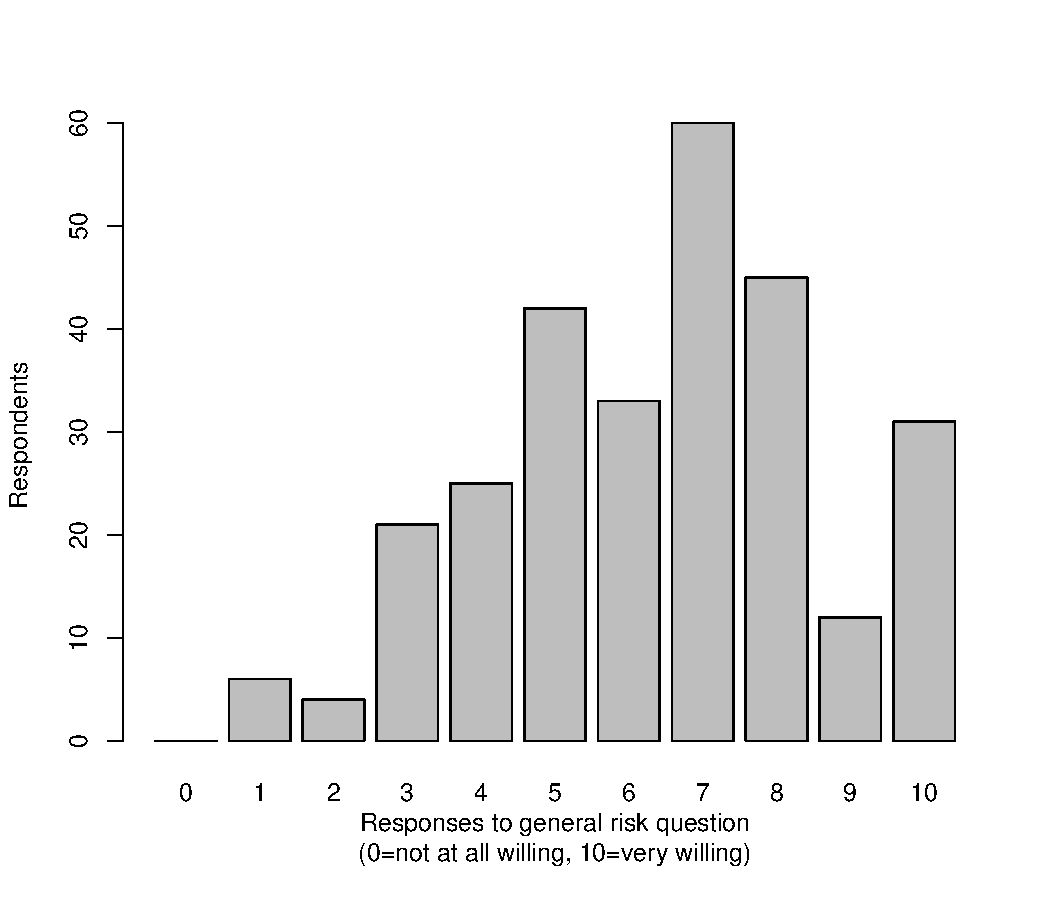
\includegraphics{Figures/risk-1.pdf}
\caption{Responses to the question about willingness to take risks ``in
general,'' measured on an eleven-point scale.}
\end{figure}

\begin{figure}
\centering
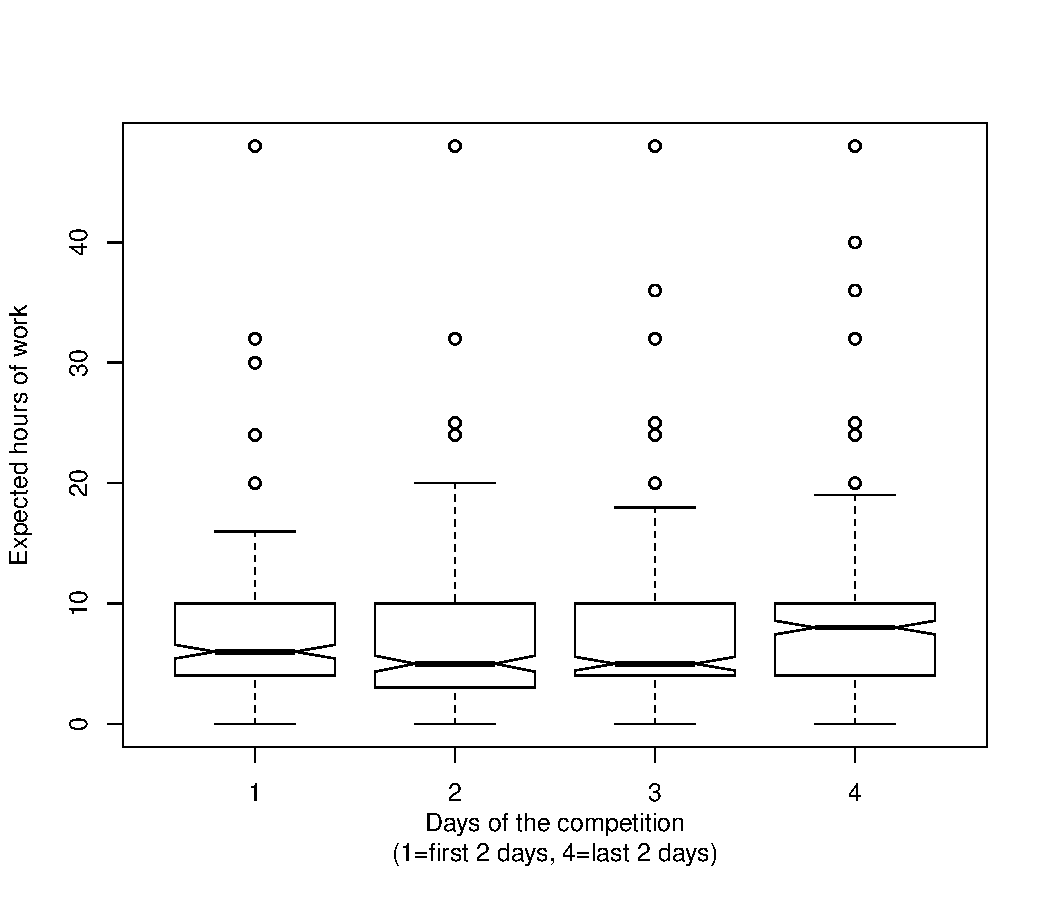
\includegraphics{Figures/looking-ahead-1.pdf}
\caption{Responses to the question about expected hours of work for
every 2 days of the competition.}
\end{figure}

\begin{figure}
\centering
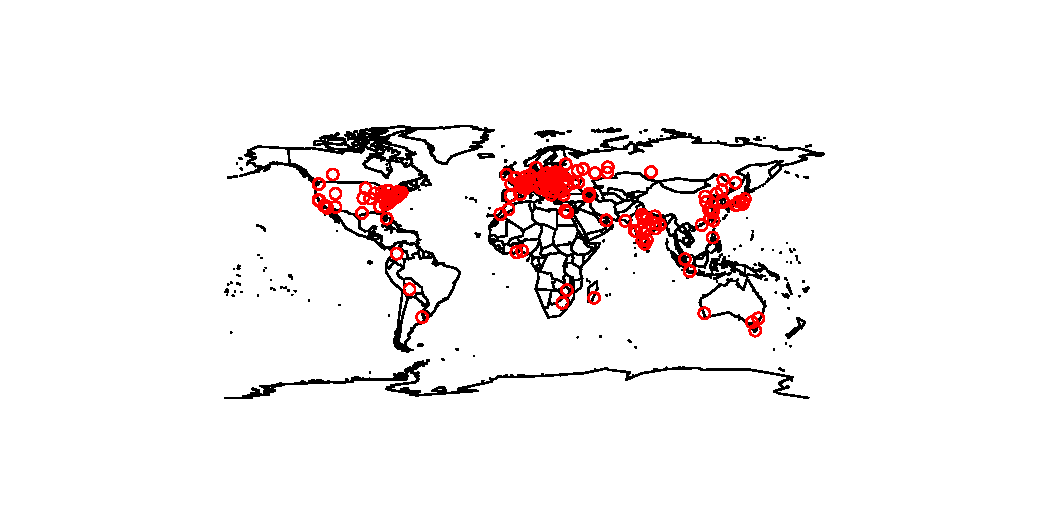
\includegraphics{Figures/unnamed-chunk-9-1.pdf}
\caption{xxxx}
\end{figure}

A total of 299 competitors signed-up to take part in the challenge. They
were all xxxx members of the platform with between NA and NA weeks as
registered members. In terms of skill ratings, the distribution was
highly skewed with competitors in the highest 90th percentile having
participated in 28 more competitions than those in the 10th percentile.
Likewise skills as measured by the individual ratings, if there was one,
had a skewed distribution with 1034 higher points than those in the 10th
percentile; see Figure \ref{eq: distribution experience}.

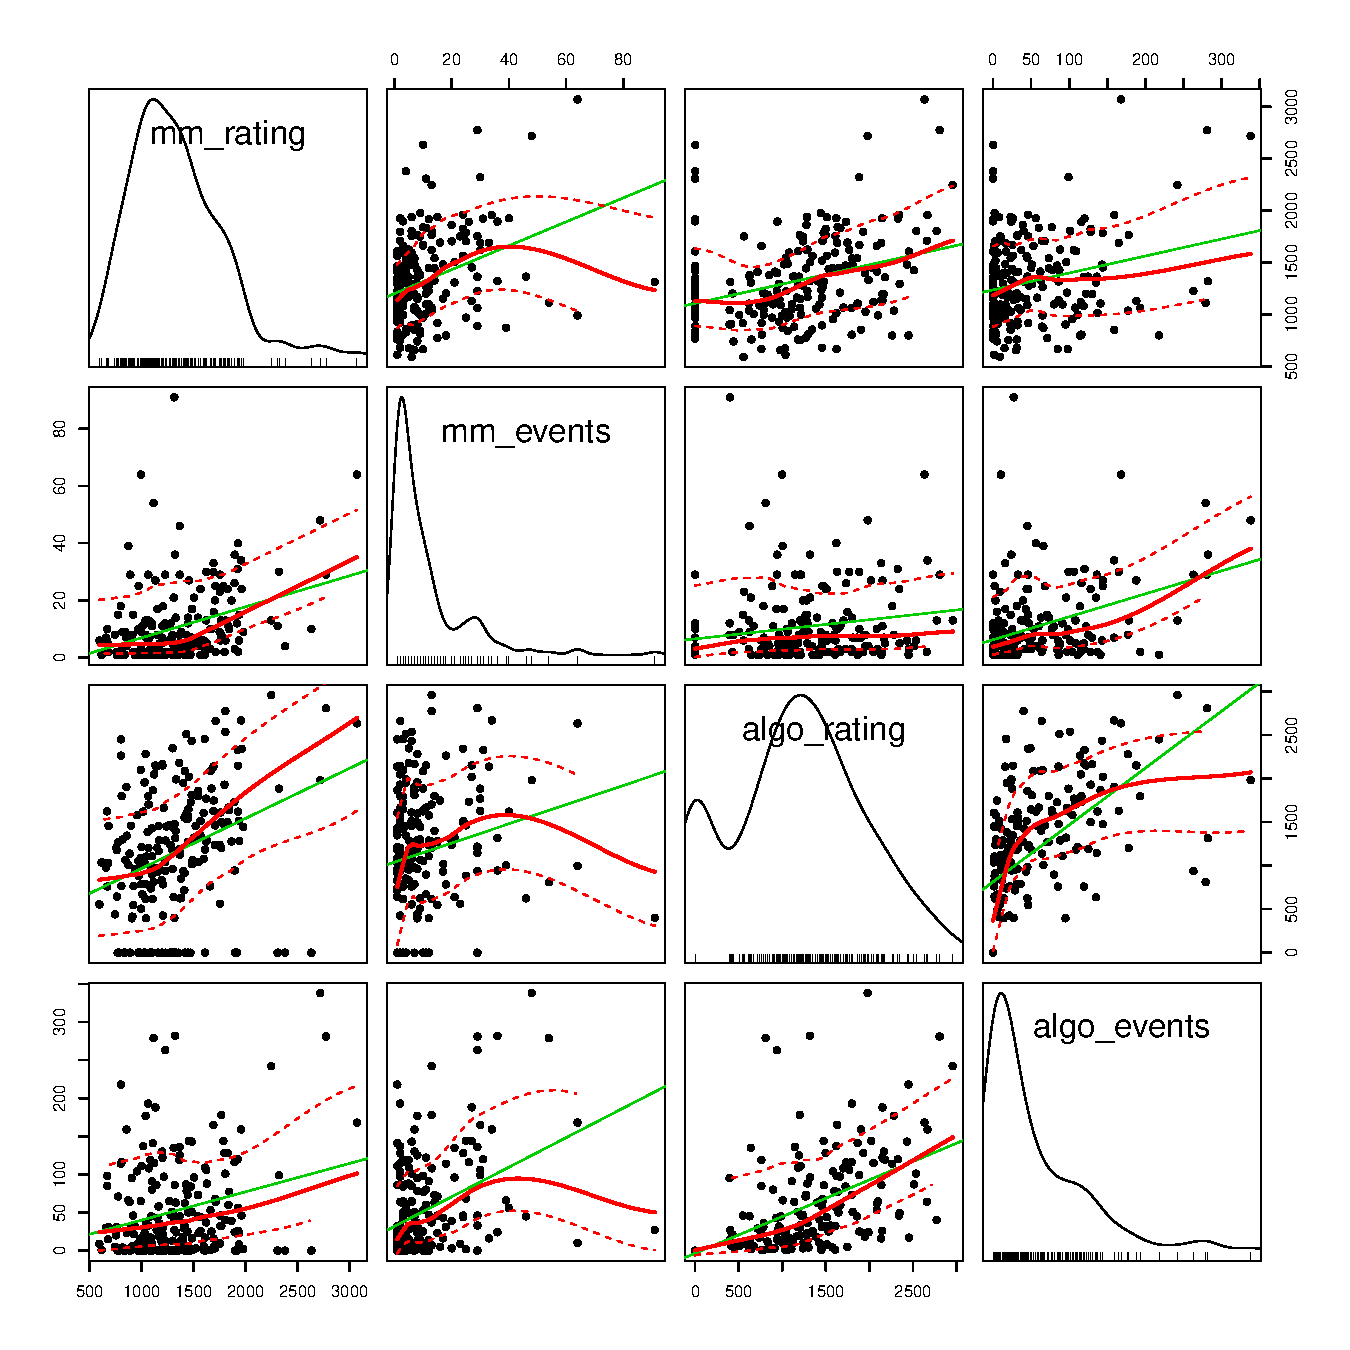
\includegraphics{Figures/ratings-1.pdf}

\section{Results}\label{results}

\begin{verbatim}
##        
##         race tournament reserve
##   FALSE   73         67      73
##   TRUE    26         33      27
\end{verbatim}

In the eight-day submission period, we collected a total of 1759
submissions made by 86 participants, with a median of 11 submissions per
person (maximum of 126 submissions). Consistent with our prediction, the
response rate was higher in the Tournament group (33 percent), followed
by the Tournament w/reseve (27 percent), and the Race treatment (26
percent). Though the association between treatment and response rates
was not statistically significant (a Fisher's Exact Test for Count Data
gives a p-value of 0.526).

\begin{verbatim}
##        
##         Large Small
##   FALSE   128    85
##   TRUE     52    34
\end{verbatim}

We find no difference between participation in large or small rooms (a
Fisher's Exact Test for Count Data gives a p-value of 1).

\begin{verbatim}
##              race tournament reserve
##                                     
## Large FALSE    44         42      42
##       TRUE     16         18      18
## Small FALSE    29         25      31
##       TRUE     10         15       9
\end{verbatim}

We also find no evidence of an overall association between treatments,
room size and participation (a Fisher's Exact Test for Count Data gives
a p-value of 0.86).

\begin{figure}
\centering
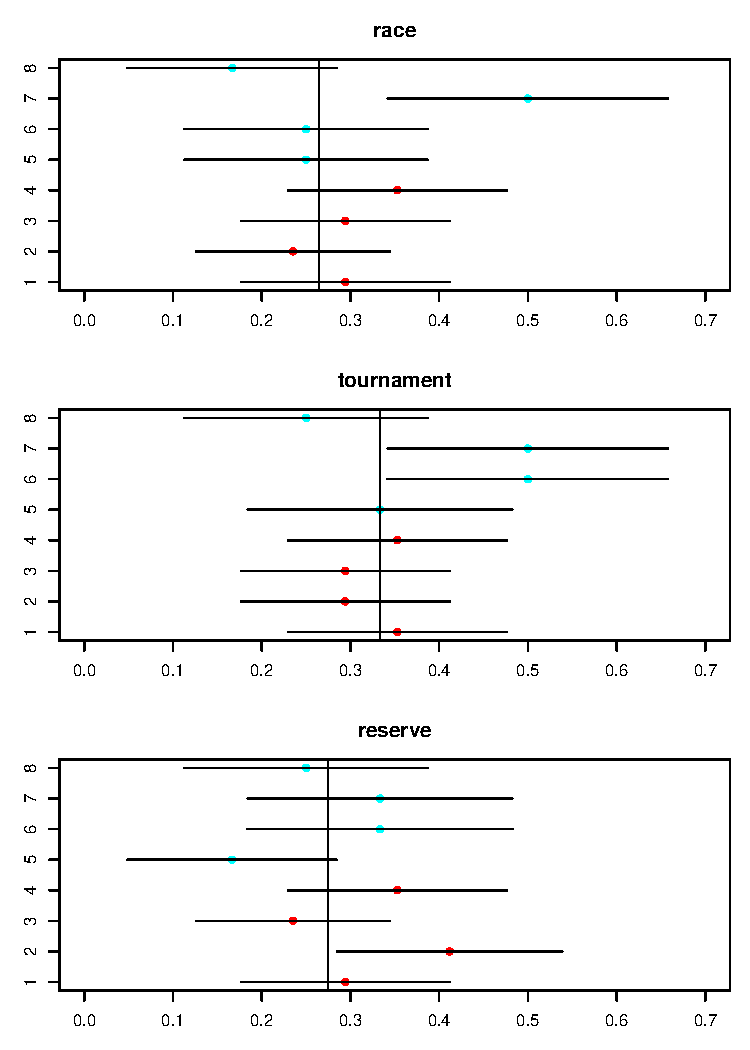
\includegraphics{Figures/unnamed-chunk-13-1.pdf}
\caption{Participation rates by rooms}
\end{figure}

\renewcommand\refname{References}
\bibliography{library.bib}

\end{document}